\section{approach}
\subsection{Approach Overview}
Our approach takes the coverage data and reported issues as input and outputs the non-covered branches with the associated issues. Figure 1 shows the high level design of Covana. Covana consists of three major components: observer component, pre-processing component and analysis component.
\\The observer is implemented as several Pex extension and is attached to Pex for observing different events and collecting data. It collects the coverage data and reported issues and passed them to the pre-processing component. The pre-processing component remove the useless data and dump the data into binary files. The analysis component consumes the pre-processed data in files, carrys out the analysis on the data and outputs the relevant data for non-covered issues.
\subsection{Observer Component}
The observer component is implemented as three Pex extensions: (1) Branch coverage observer. (2) Field access observer. (3) Issues observer.
\subsubsection{Branch coverage observer}
The branch coverage observer is attached to Pex for collecting the branch coverage data. After all the generated tests are executed, it will enumerate the methods of the class under test, checks the coverage information of each branch inside a method and find out the non-covered branches. As Pex runs on top of MSIL (MicroSoft Intermediate Language) assembly, the observer also collects the IL offset of each non-covered branches for further analysis.
\subsubsection{Field access observer}

\subsubsection{Issues observer}
The issue observer collects different kinds of issues reported by Pex, such as object creation issues, uninstrumented method issues and testability issues.

\subsection{Pre-processing Component}
The pre-processing component pre-processed the different kinds of data collected by the observer component and filter out the useless data based on some heuristics.
\subsubsection{Filter out useless branch coverage data}
Not all the collected non-covered branches are useful for user to look at \ref{sample}. 

\begin{figure}[t]
\begin{CodeOut}
\begin{alltt}
\begin{scriptsize}
if (x != null) \{
   Console.WriteLine("type: " + x.GetType());
\}
IEnumerator xe = x.GetEnumerator();
\end{scriptsize}
\end{alltt}
\end{CodeOut}
\Caption{\label{fig:intstack}An integer stack implementation}
\end{figure}

%\begin{figure}%
%\includegraphics[scale=0.4, trim=0 120mm 100mm 0mm]{code1.eps}%l b r t
%\caption{}%
%\label{sample}5t
%\end{figure}

%\begin{figure}%
%\begin{CodeOut}
%\begin{alltt}
%
%\end{alltt}
%
%\end{CodeOut}\caption{}%
%\label{}%
%\end{figure}